% This is "sig-alternate.tex" V2.1 April 2013
% This file should be compiled with V2.5 of "sig-alternate.cls" May 2012
%
% This example file demonstrates the use of the 'sig-alternate.cls'
% V2.5 LaTeX2e document class file. It is for those submitting
% articles to ACM Conference Proceedings WHO DO NOT WISH TO
% STRICTLY ADHERE TO THE SIGS (PUBS-BOARD-ENDORSED) STYLE.
% The 'sig-alternate.cls' file will produce a similar-looking,
% albeit, 'tighter' paper resulting in, invariably, fewer pages.
%
% ----------------------------------------------------------------------------------------------------------------
% This .tex file (and associated .cls V2.5) produces:
%       1) The Permission Statement
%       2) The Conference (location) Info information
%       3) The Copyright Line with ACM data
%       4) NO page numbers
%
% as against the acm_proc_article-sp.cls file which
% DOES NOT produce 1) thru' 3) above.
%
% Using 'sig-alternate.cls' you have control, however, from within
% the source .tex file, over both the CopyrightYear
% (defaulted to 200X) and the ACM Copyright Data
% (defaulted to X-XXXXX-XX-X/XX/XX).
% e.g.
% \CopyrightYear{2007} will cause 2007 to appear in the copyright line.
% \crdata{0-12345-67-8/90/12} will cause 0-12345-67-8/90/12 to appear in the copyright line.
%
% ---------------------------------------------------------------------------------------------------------------
% This .tex source is an example which *does* use
% the .bib file (from which the .bbl file % is produced).
% REMEMBER HOWEVER: After having produced the .bbl file,
% and prior to final submission, you *NEED* to 'insert'
% your .bbl file into your source .tex file so as to provide
% ONE 'self-contained' source file.
%
% ================= IF YOU HAVE QUESTIONS =======================
% Questions regarding the SIGS styles, SIGS policies and
% procedures, Conferences etc. should be sent to
% Adrienne Griscti (griscti@acm.org)
%
% Technical questions _only_ to
% Gerald Murray (murray@hq.acm.org)
% ===============================================================
%
% For tracking purposes - this is V2.0 - May 2012

\documentclass{sig-alternate-05-2015}
\usepackage{graphicx}
\usepackage{subfigure}
\usepackage{times}

\begin{document}

% Copyright
\setcopyright{acmcopyright}
%\setcopyright{acmlicensed}
%\setcopyright{rightsretained}
%\setcopyright{usgov}
%\setcopyright{usgovmixed}
%\setcopyright{cagov}
%\setcopyright{cagovmixed}


% DOI
\doi{10.475/123_4}

% ISBN
\isbn{123-4567-24-567/08/06}

%Conference
\conferenceinfo{PLDI '13}{June 16--19, 2013, Seattle, WA, USA}

\acmPrice{\$15.00}

%
% --- Author Metadata here ---
\conferenceinfo{WOODSTOCK}{'97 El Paso, Texas USA}
%\CopyrightYear{2007} % Allows default copyright year (20XX) to be over-ridden - IF NEED BE.
%\crdata{0-12345-67-8/90/01}  % Allows default copyright data (0-89791-88-6/97/05) to be over-ridden - IF NEED BE.
% --- End of Author Metadata ---

\title{Lessons Learned from Validating\\ Industrial Text Mining Methods \titlenote{(Produces the permission block, and
copyright information). For use with
SIG-ALTERNATE.CLS. Supported by ACM}}
 
%
% You need the command \numberofauthors to handle the 'placement
% and alignment' of the authors beneath the title.
%
% For aesthetic reasons, we recommend 'three authors at a time'
% i.e. three 'name/affiliation blocks' be placed beneath the title.
%
% NOTE: You are NOT restricted in how many 'rows' of
% "name/affiliations" may appear. We just ask that you restrict
% the number of 'columns' to three.
%
% Because of the available 'opening page real-estate'
% we ask you to refrain from putting more than six authors
% (two rows with three columns) beneath the article title.
% More than six makes the first-page appear very cluttered indeed.
%
% Use the \alignauthor commands to handle the names
% and affiliations for an 'aesthetic maximum' of six authors.
% Add names, affiliations, addresses for
% the seventh etc. author(s) as the argument for the
% \additionalauthors command.
% These 'additional authors' will be output/set for you
% without further effort on your part as the last section in
% the body of your article BEFORE References or any Appendices.

\numberofauthors{2} %  in this sample file, there are a *total*
% of EIGHT authors. SIX appear on the 'first-page' (for formatting
% reasons) and the remaining two appear in the \additionalauthors section.
%
\author{
% You can go ahead and credit any number of authors here,
% e.g. one 'row of three' or two rows (consisting of one row of three
% and a second row of one, two or three).
%
% The command \alignauthor (no curly braces needed) should
% precede each author name, affiliation/snail-mail address and
% e-mail address. Additionally, tag each line of
% affiliation/address with \affaddr, and tag the
% e-mail address with \email.
%
% 1st. author
\alignauthor
Zhe Yu, Rahul Krishna, \\Amritanshu Agrawa, Tim Menzies\titlenote{}\\
       \affaddr{Institute for Clarity in Documentation}\\
       \affaddr{1932 Wallamaloo Lane}\\
       \affaddr{Wallamaloo, New Zealand}\\
       \email{zyu9@ncsu.edu}
% 2nd. author
\alignauthor
Manuel Dominguez,\\ David Wolf \titlenote{}\\
       \affaddr{Institute for Clarity in Documentation}\\
       \affaddr{P.O. Box 1212}\\
       \affaddr{Dublin, Ohio 43017-6221}\\
       \email{webmaster@marysville-ohio.com}
}

% Just remember to make sure that the TOTAL number of authors
% is the number that will appear on the first page PLUS the
% number that will appear in the \additionalauthors section.

\maketitle
\begin{abstract}

Just a skeleton... should have all the figures at the end of today...

\end{abstract}


%
% The code below should be generated by the tool at
% http://dl.acm.org/ccs.cfm
% Please copy and paste the code instead of the example below. 
%
\begin{CCSXML}
<ccs2012>
 <concept>
  <concept_id>10010520.10010553.10010562</concept_id>
  <concept_desc>Computer systems organization~Embedded systems</concept_desc>
  <concept_significance>500</concept_significance>
 </concept>
 <concept>
  <concept_id>10010520.10010575.10010755</concept_id>
  <concept_desc>Computer systems organization~Redundancy</concept_desc>
  <concept_significance>300</concept_significance>
 </concept>
 <concept>
  <concept_id>10010520.10010553.10010554</concept_id>
  <concept_desc>Computer systems organization~Robotics</concept_desc>
  <concept_significance>100</concept_significance>
 </concept>
 <concept>
  <concept_id>10003033.10003083.10003095</concept_id>
  <concept_desc>Networks~Network reliability</concept_desc>
  <concept_significance>100</concept_significance>
 </concept>
</ccs2012>  
\end{CCSXML}

\ccsdesc[500]{Computer systems organization~Embedded systems}
\ccsdesc[300]{Computer systems organization~Redundancy}
\ccsdesc{Computer systems organization~Robotics}
\ccsdesc[100]{Networks~Network reliability}


%
% End generated code
%

%
%  Use this command to print the description
%
\printccsdesc

% We no longer use \terms command
%\terms{Theory}

\keywords{Software Engineering; text mining}

\section{Introduction}

The main purpose of this paper is to build a baseline result for text mining in Software Engineering. There has been little work for mining the text in Software Engineering, among which the StackOverflow data is most commonly used. StackOverflow is a part of StackExchange, the biggest Question \& Answer website, and it is constructed especially for software engineers. Thousands of software engineers ask questions or search for answers on StackOverflow everyday. The tag for posts on StackOverflow is a key feature to facilitate the answering and searching process. Mining the StackOverflow posts to predict tags can save the time and effort of users of tagging their posts. Several approaches have been discussed to predict tags on StackOverflow \cite{stanley2013predicting,moharanatag,kuo2011word}, but there has been little effort of how to evaluate the performance and no solid baseline result has been built.

Predicting tags is a multi-classification and multi-label task. To simplify the experiment and to make comparisons easier, only one tag is kept for each post. The original problem is then transformed into a multi-classification one. A framework of text mining for Software Engineering is constructed and various of decisions are explored to find the best practice of this task in the scope of current general text mining techniques. To contribute to the research of text mining in Software Engineering, the following research questions are answered in this paper.

\textbf{RQ1} Where should we focus our exploration and which decisions have we explored?

\textbf{RQ2} What is the proper performance metric for this multi-classification task?

\textbf{RQ3} What is the best practice for this task?

\textbf{RQ4} How can we further improve the performance?

The first two research questions, \textbf{RQ1} and \textbf{RQ2}, are answered in Section \ref{sec:Method}. \textbf{RQ3} is answered in Section \ref{sec:Experiment} and \textbf{RQ4} is answered in Section \ref{sec:Discussion}.

\subsection{Data}

\begin{figure}[ht]
  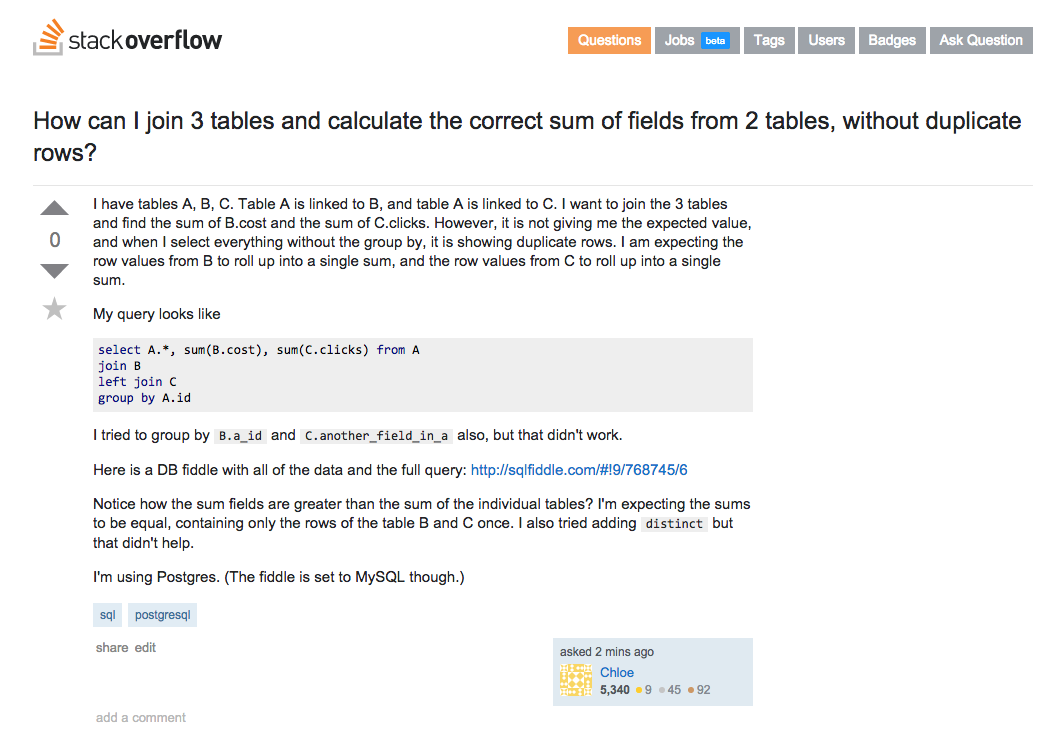
\includegraphics[width=\linewidth]{./fig/example.png}
  \caption{StackOverflow Post}
  \label{fig:example}
\end{figure}

Data is gathered from https://archive.org/details/stackexchange. An example of StackOverflow post is shown in Figure \ref{fig:example}. Twenty data sets generated from StackOverflow posts are used in the experiments. Each data set contains ten thousand posts. The title and body of the posts are concatenated to form the independent variables for classification. The first tag for the posts are treated as the class of the post. The distribution of classes is shown Figure \ref{fig:classes}. Since many classes have such a small population, only the classes with top 19 population are kept while all the other classes are combined into one single class 'others'.

\begin{figure}[ht]
  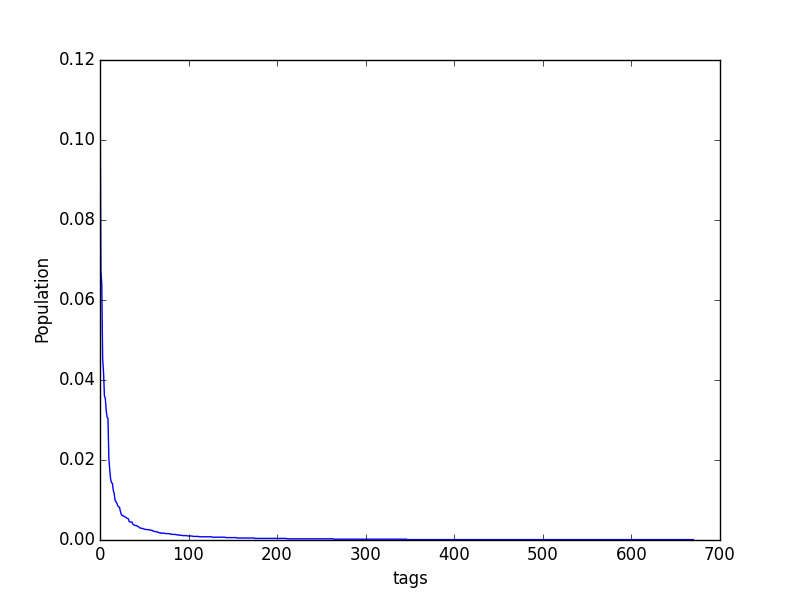
\includegraphics[width=\linewidth]{./fig/classes.png}
  \caption{Class distribution}
  \label{fig:classes}
\end{figure}

\subsection{Related works}

Moharana, 2013 \cite{moharanatag} has tried different approaches to predict StackOverflow tags. Three different classifiers, Linear SVM, Multinomial Naive Bayes, and Perceptron, with two different features, term frequency and tf-idf, are tested. The performance is meatured by $F_{1}$ score. However, the definition of $F_{1}$ score is ambiguous because of the multi-classification task. Best approach in \cite{moharanatag} is linear SVM + tf-idf and the $F_{1}$ score is $0.5358$.

Clayton and Byrne, 2013 \cite{stanley2013predicting} have worked on StackOverflow tag prediction and developed an ACT-R inspired Bayesian probabilistic model. This approach achieves a $65\%$ of accuracy by choosing the tag that has the highest log odds of being correct, given the tag’s prior log odds of occurrence and adjusting for the log likelihood ratio of the words in the post being associated with the tag.

Kuo, 2011 \cite{kuo2011word} has also worked on StackOverflow tag prediction. Kuo uses a co-occurrence model that predicts tags based on the relation (co-occurrence) between the words and tags. Initially built for next-word prediction in large documents, this model is adapted to the StackOverflow dataset by constraining the next word predicted to only tags. A $47\%$ classification accuracy is achieved.

Another model called SNIF-ACT (Fu \& Pirolli, 2007 \cite{fu2007snif}) also uses co-occurrences and can predict link traversal for search queries. The model predicts the most likely link that a person will click on by a search query (goal state) and fetched results. 


\section{Method}
\label{sec:Method}

\textbf{RQ1} Where should we focus our exploration and which decisions have we explored?

A greedy search is implemented on the following decisions:

\textbf{Tokenization:} a) bag of words; b) stemming and stop words removal.

\textbf{Featurization:} a) term frequency; b) tf-idf.

\textbf{Normalization:} a) L2 normalization on rows; b) L2 normalization on columns; c) do not do normalization.

\textbf{Dimensionality Reduction:} a) Hashing trick; b) tf-idf selection.

\textbf{Data Balancing:} a) SMOTE as oversampling method and sample without replacement as under-sampling method; b) do not balance the data.

\textbf{Classification:} a) Linear SVM; b) Multinomial Naive Bayes; c) CART as decision tree.

\subsection{Performance Metrics}

For each experiment, all three of the following scores are calculated:

\textbf{Accuracy:} accuracy always has its own problem...

\textbf{$Fscore_{M}$:} F-score on each tag can be calculated after the trained classifier is tested on test set. The mean of F-score on each tag is then calculated to represent the overall performance of the classifier. Regardless of the population within each tag, the $Fscore_{M}$ represents performance on each tag equally \cite{sokolova2009systematic}.

\textbf{$Fscore_{\mu}$:} the $Fscore_{\mu}$ on each tag is calculated by multiply F-score on each tag by its population. Classifiers are trained to achieve high in this score by default. This score can be misleading if each tag is of the same importance \cite{sokolova2009systematic}.

\textbf{RQ2} What is the proper performance metric for this multi-classification task?

While most of the current approaches favor accuracy as their performance metric \cite{stanley2013predicting,kuo2011word}, we prefer $Fscore_{M}$. Justifications...

\section{Experiment}
\label{sec:Experiment}

For each experiment, a 5 by 5 cross-validation ($80\%$ as training sample and $20\%$ as testing sample) is performed on 20 data sets (each has ten thousand posts).

\subsection{Best Practice}

\textbf{RQ3} What is the best practice for this task?

The best practice we suggest is:

\textbf{Tokenization:} bag of words.

\textbf{Featurization:} term frequency.

\textbf{Normalization:} L2 normalization on rows.

\textbf{Dimensionality Reduction:} tf-idf selection, 4000 features.

\textbf{Data Balancing:} SMOTE as oversampling method and sample without replacement as under-sampling method.

\textbf{Classification:} Linear SVM.

\begin{figure}[ht]
  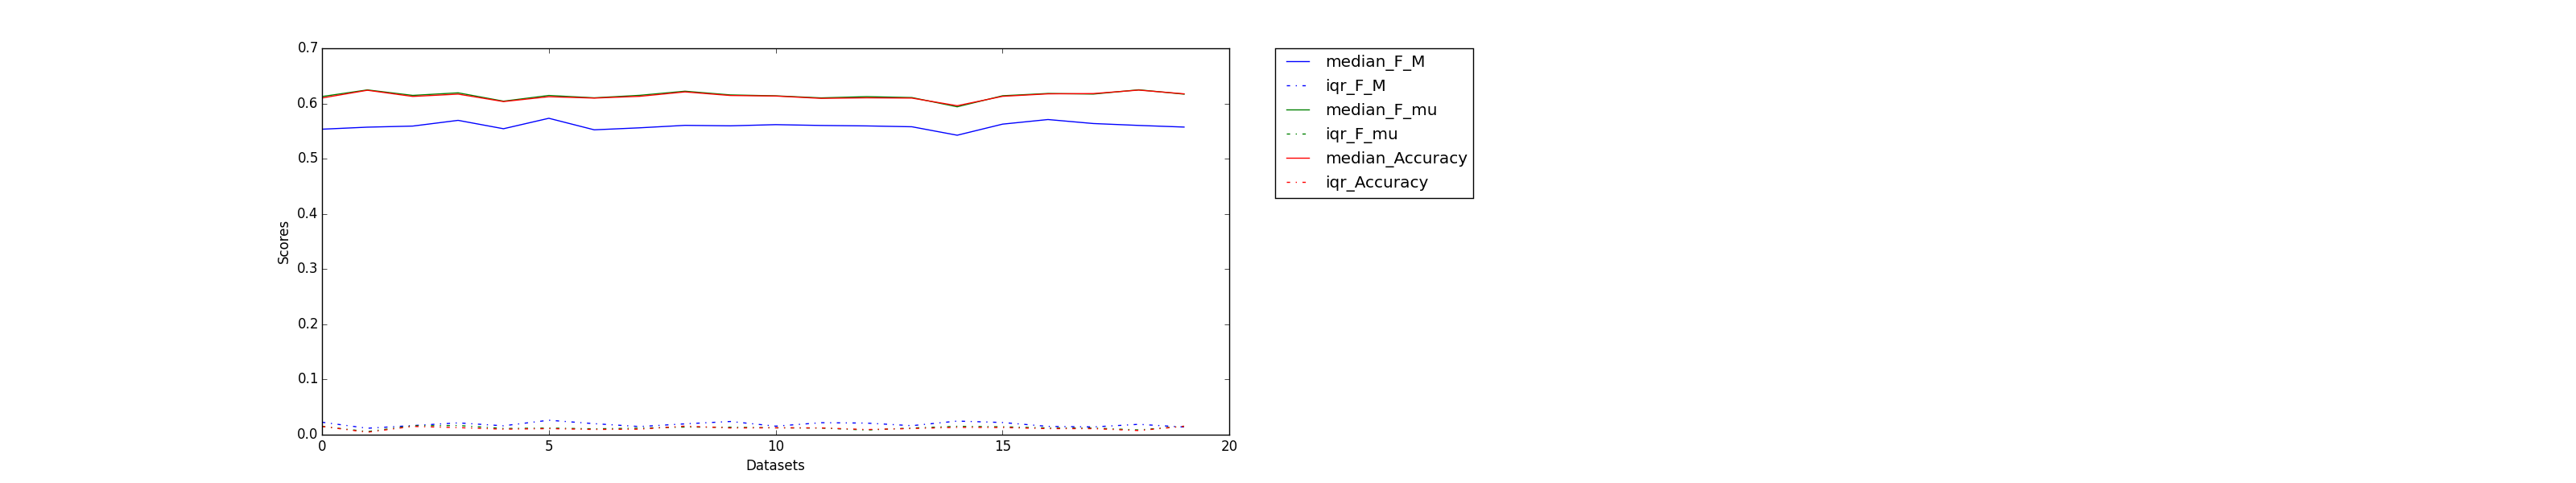
\includegraphics[width=\linewidth]{./fig/best.png}
  \caption{Best Practice}
  \label{fig:best}
\end{figure}

The performance of the best practice is: accuracy: 0.613, $Fscore_{M}$: 0.560, $Fscore_{\mu}$: 0.614, as shown in Figure \ref{fig:best}. 

\subsection{Tokenization Decisions}

Stemming and stop words removal are considered as an effective way to improve the text classification performance \cite{yang1997comparative}. However contradictory evidences show that in the task of predicting tags, Stemming and stop words removal are not preferred \cite{moharanatag,stanley2013predicting}.

\begin{figure}[ht]
    \centering
    \subfigure[$Accuracy$]
    {
        \includegraphics[width=\linewidth]{./fig/stem_acc.png}
        \label{fig:stem_acc}
    }
    \quad
    \subfigure[$Fscore_{M}$]
    {
        \includegraphics[width=\linewidth]{./fig/tem_M.png}
        \label{fig:stem_M}
    }
    \quad
    \subfigure[$Fscore_{\mu}$]
    {
        \includegraphics[width=\linewidth]{./fig/tem_mu.png}
        \label{fig:stem_mu}
    }
    \caption{Stemming versus no stemming}
    \label{fig:stem}
\end{figure}

As shown in Figure \ref{fig:stem}, stemming and stop words removal has no improvements on the performance. Therefore doing nothing, keeping the original bag of words is recommended.

\subsection{Featurization Decisions}

Tf-idf weight has been a popular feature for text categorization for years \cite{caropreso2001learner} and it is suggested in \cite{moharanatag} that better performance can be achieved with it. On the other hand, term frequency is the simplest and most common used feature for text categorization. It is necessary to compare these two features in this task.

\begin{figure}[ht]
    \centering
    \subfigure[$Accuracy$]
    {
        \includegraphics[width=\linewidth]{./fig/fea_acc.png}
        \label{fig:fea_acc}
    }
    \quad
    \subfigure[$Fscore_{M}$]
    {
        \includegraphics[width=\linewidth]{./fig/fea_M.png}
        \label{fig:fea_M}
    }
    \quad
    \subfigure[$Fscore_{\mu}$]
    {
        \includegraphics[width=\linewidth]{./fig/fea_mu.png}
        \label{fig:fea_mu}
    }
    \caption{term frequency versus tf-idf}
    \label{fig:fea}
\end{figure}

As shown in Figure \ref{fig:fea}, term frequency performs slightly better than tf-idf. Therefore term frequency is recommended for featurization.

\subsection{Normalization Decisions}

L2 normalization on rows is the standard normalization method for text categorization \cite{frank2006naive}. The main purpose of implementing L2 normalization on rows is to normalize each document to unit length. L2 normalization on columns is more common to see in other data mining tasks. The main purpose of implementing L2 normalization on columns is to normalize each feature to same weight. 

\begin{figure}[ht]
    \centering
    \subfigure[$Accuracy$]
    {
        \includegraphics[width=\linewidth]{./fig/norm_acc.png}
        \label{fig:norm_acc}
    }
    \quad
    \subfigure[$Fscore_{M}$]
    {
        \includegraphics[width=\linewidth]{./fig/norm_M.png}
        \label{fig:norm_M}
    }
    \quad
    \subfigure[$Fscore_{\mu}$]
    {
        \includegraphics[width=\linewidth]{./fig/norm_mu.png}
        \label{fig:norm_mu}
    }
    \caption{L2 normalization on rows versus on columns versus no normalization}
    \label{fig:norm}
\end{figure}

As shown in Figure \ref{fig:norm}, L2 normalization on rows outperforms others. Therefore L2 normalization on rows is recommended for normalization.

\subsection{Dimensionality Reduction Decisions}

Hashing is considered as an effective strategy for dimensionality reduction \cite{weinberger2009feature}. Feature selection by tf-idf score is also discussed in literature as an excellent method for text categorization \cite{menzies2006improving}.

\begin{figure}[ht]
    \centering
    \subfigure[$Accuracy$]
    {
        \includegraphics[width=\linewidth]{./fig/sel_acc.png}
        \label{fig:sel_acc}
    }
    \quad
    \subfigure[$Fscore_{M}$]
    {
        \includegraphics[width=\linewidth]{./fig/sel_M.png}
        \label{fig:sel_M}
    }
    \quad
    \subfigure[$Fscore_{\mu}$]
    {
        \includegraphics[width=\linewidth]{./fig/sel_mu.png}
        \label{fig:sel_mu}
    }
    \caption{Hashing versus tf-idf selection}
    \label{fig:sel}
\end{figure}

As shown in Figure \ref{fig:sel}, tf-idf selection performs slightly better than hashing. Therefore tf-idf selection is recommended for dimensionality reduction.

\begin{figure}[ht]
  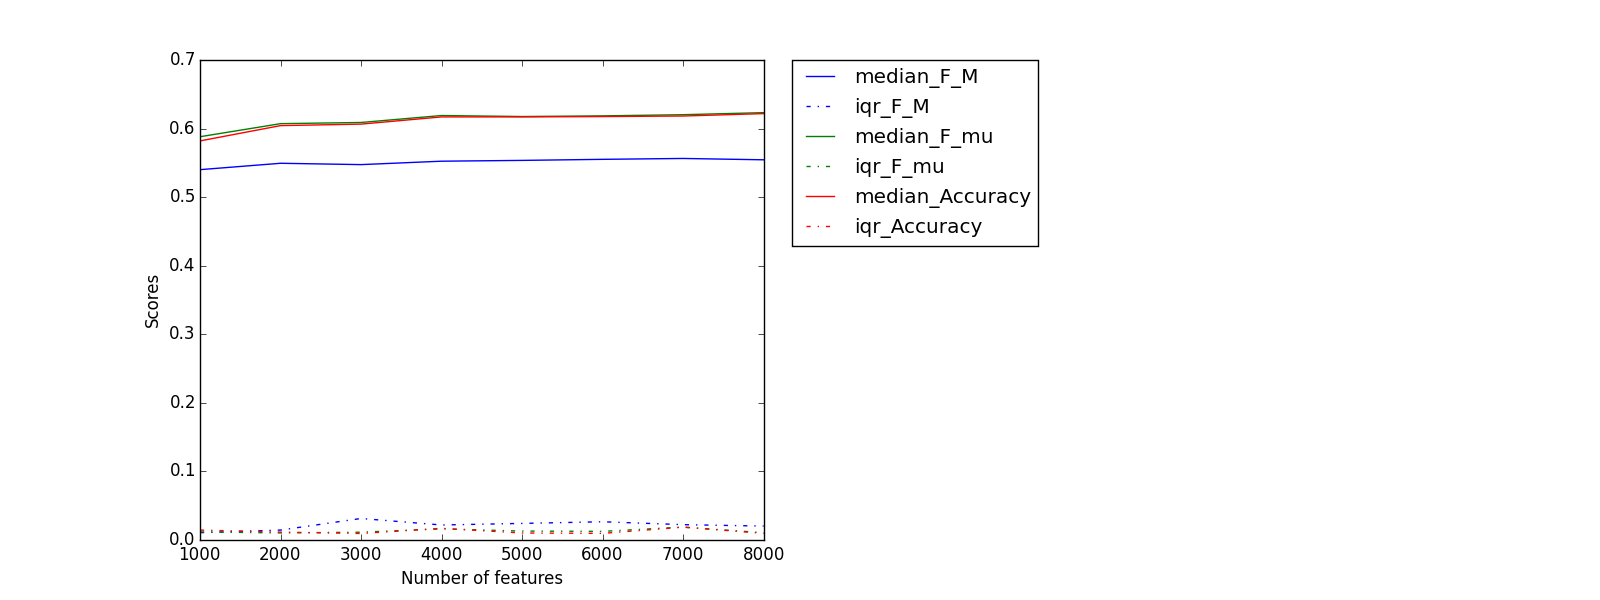
\includegraphics[width=\linewidth]{./fig/fea_num.png}
  \caption{Feature Numbers}
  \label{fig:fea_num}
\end{figure}

As shown in Figure \ref{fig:fea_num}, four thousand features are enough.

\subsection{Data Balancing Decisions}

Proposed in 2002 \cite{chawla2002smote}, SMOTE is a very effective method for balancing imbalance data and has been widely applied during the past decades \cite{han2005borderline,bunkhumpornpat2009safe,luengo2011addressing}. Given the fact that each multi-classification problem is imbalance with one versus rest approach, SMOTE can be helpful to address more weight on classes with small population.

\begin{figure}[ht]
    \centering
    \subfigure[$Accuracy$]
    {
        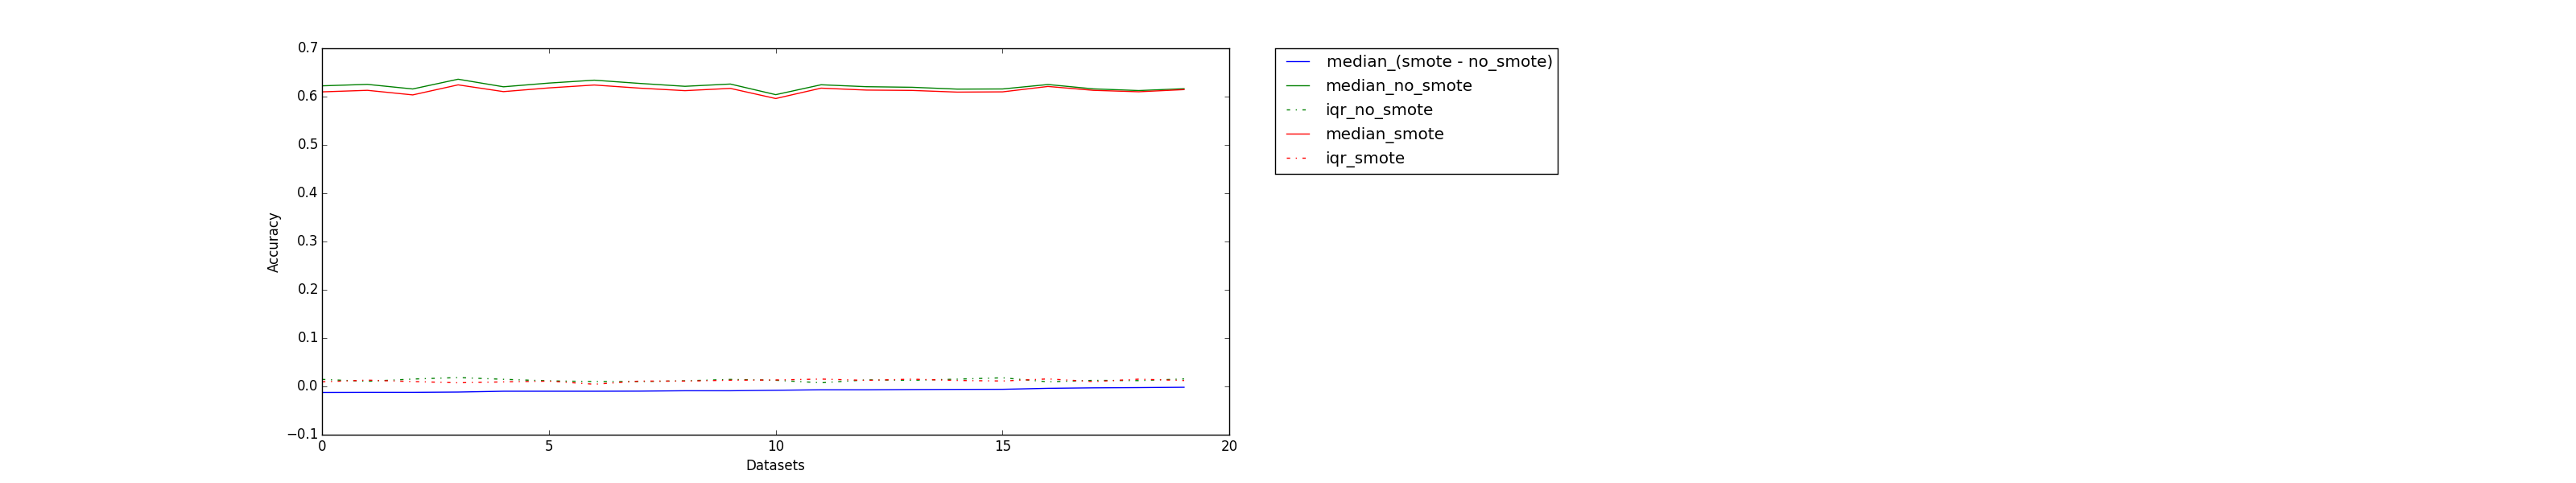
\includegraphics[width=\linewidth]{./fig/SVM_acc.png}
        \label{fig:SVM_acc}
    }
    \quad
    \subfigure[$Fscore_{M}$]
    {
        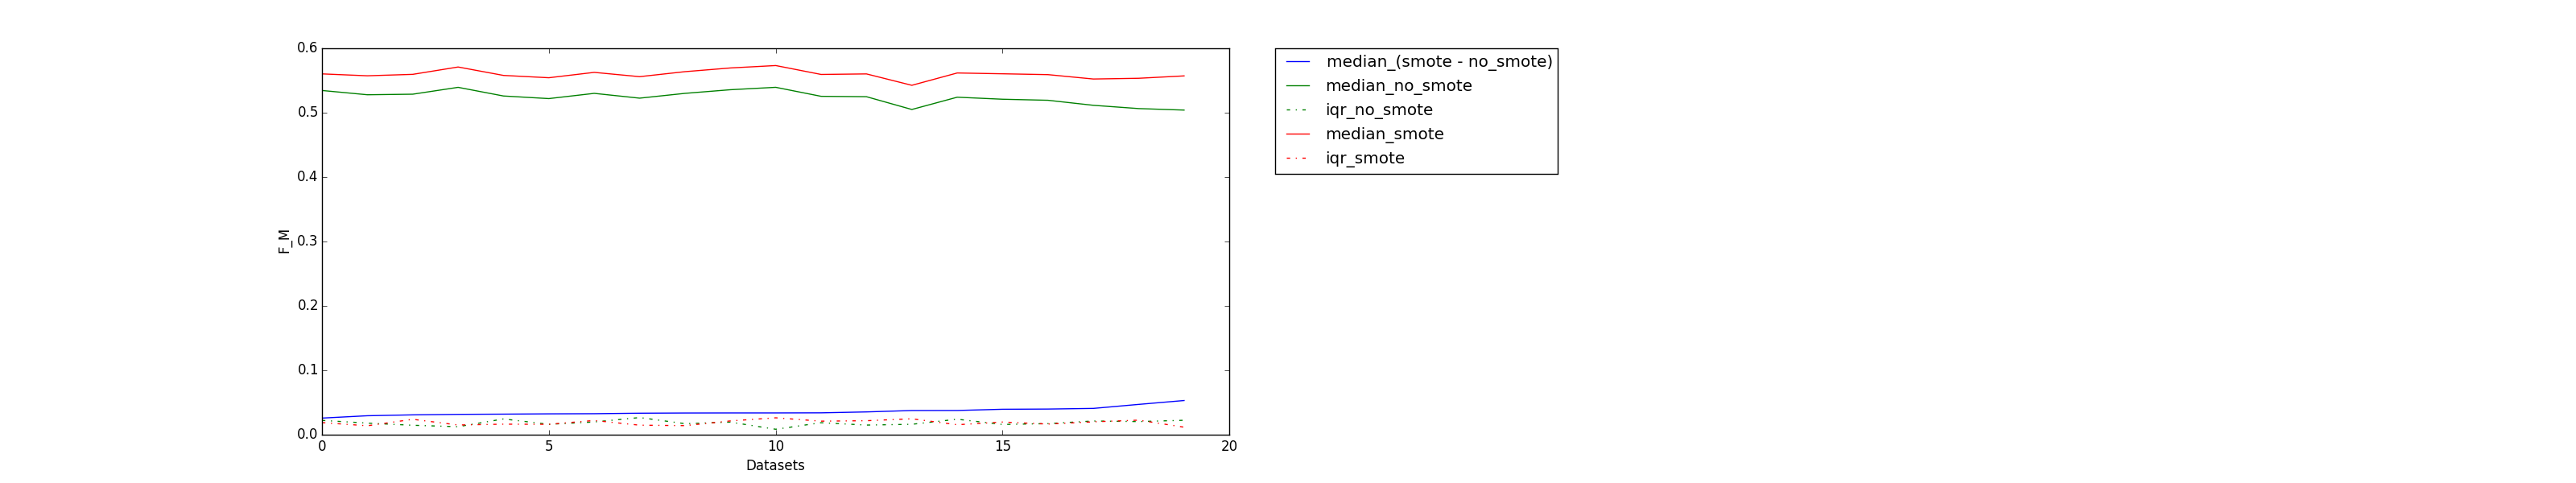
\includegraphics[width=\linewidth]{./fig/SVM_M.png}
        \label{fig:SVM_M}
    }
    \quad
    \subfigure[$Fscore_{\mu}$]
    {
        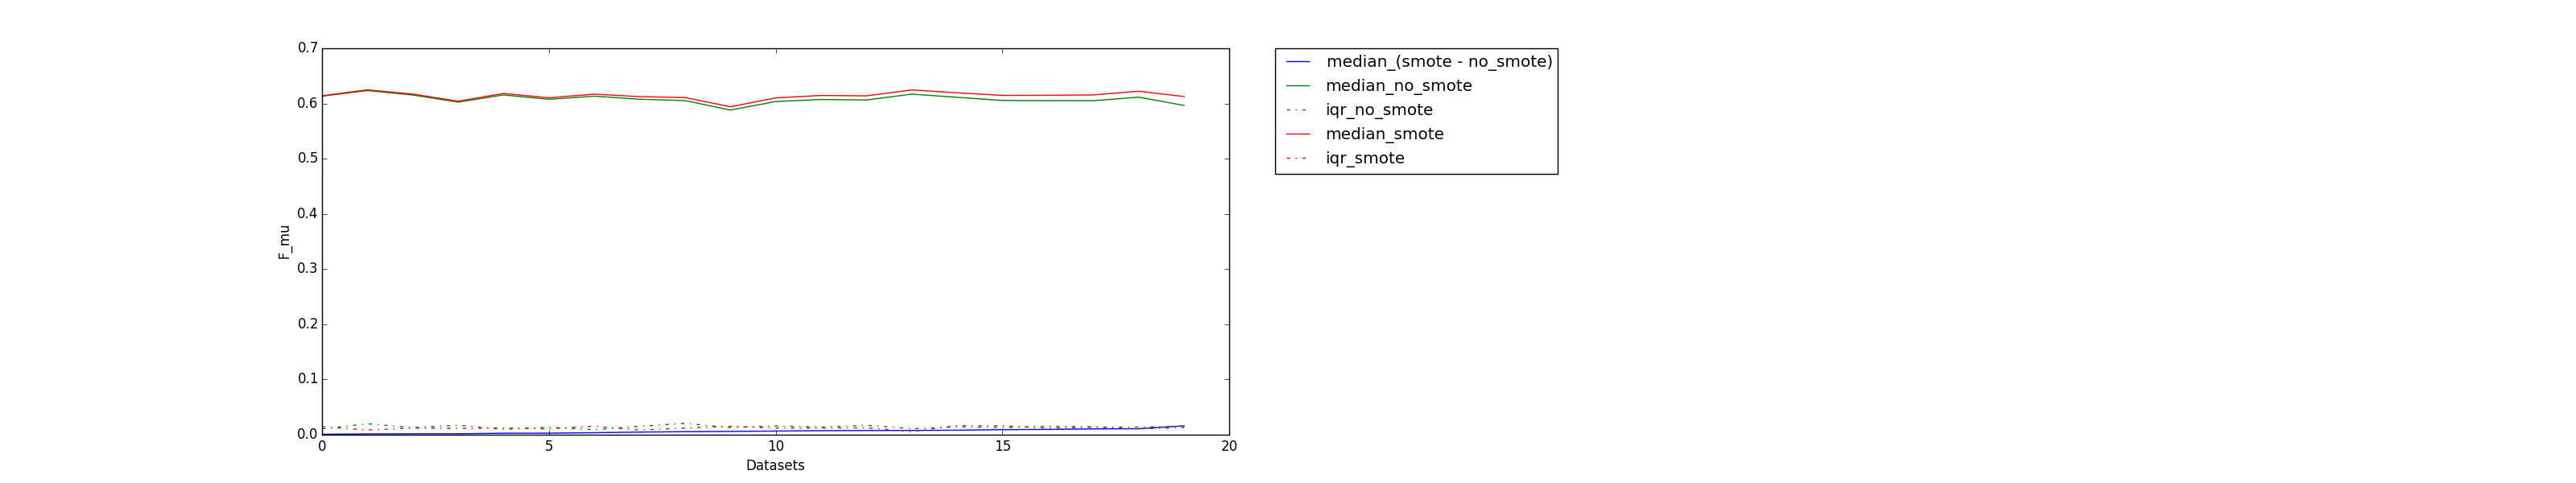
\includegraphics[width=\linewidth]{./fig/SVM_mu.png}
        \label{fig:SVM_mu}
    }
    \caption{SMOTE versus no SMOTE}
    \label{fig:SVM}
\end{figure}

As shown in Figure \ref{fig:SVM}, $Fscore_{M}$ improves after SMOTE while accuracy and $Fscore_{M}$ keeps the same. This is because SMOTE increases the weight of classes with small population, and thus causes an increase of performance on these classes and a decrease of performance on classes with large population, as shown in Figure \ref{fig:SVM_tags}.

\begin{figure}[ht]
  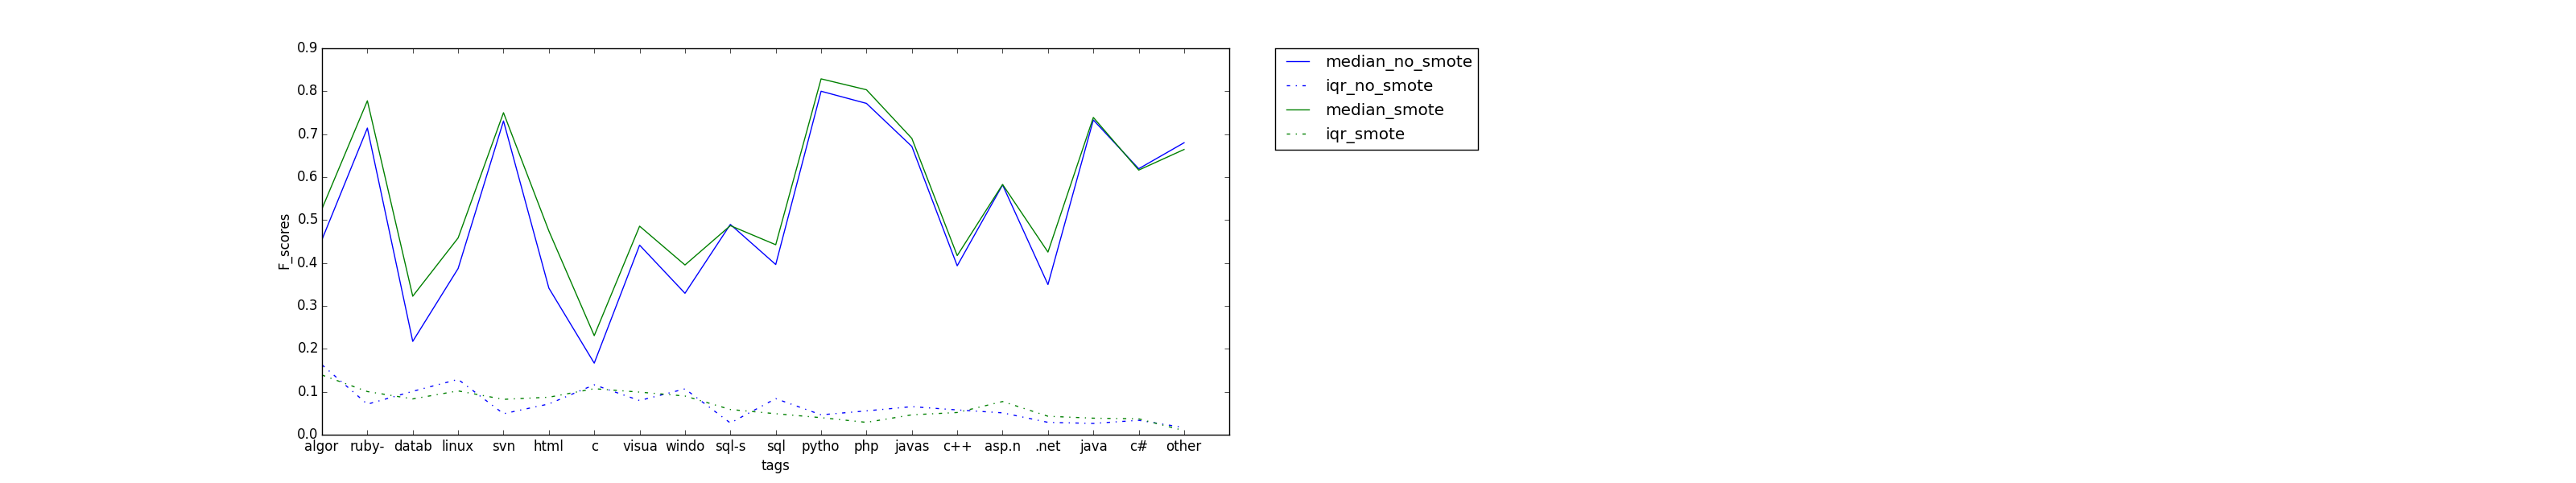
\includegraphics[width=\linewidth]{./fig/SVM_tags.png}
  \caption{F score on different classes, sorted by the population (from smallest to largest)}
  \label{fig:SVM_tags}
\end{figure}

SMOTE is suggested for data balancing since $Fscore_{M}$ is what we care most.

\subsection{Classification Decisions}

Linear SVM is one of the most common classifier for text categorization \cite{joachims2006training} and is considered the best classifier in predicting tags \cite{moharanatag}. Multinomial Naive Bayes is especially designed for text categorization \cite{mccallum1998comparison}. Another popular classifier for the comparison is decision tree. CART has been proved to be a good choice of decision tree in \cite{miotto2005supporting}.

\begin{figure}[ht]
    \centering
    \subfigure[$Accuracy$]
    {
        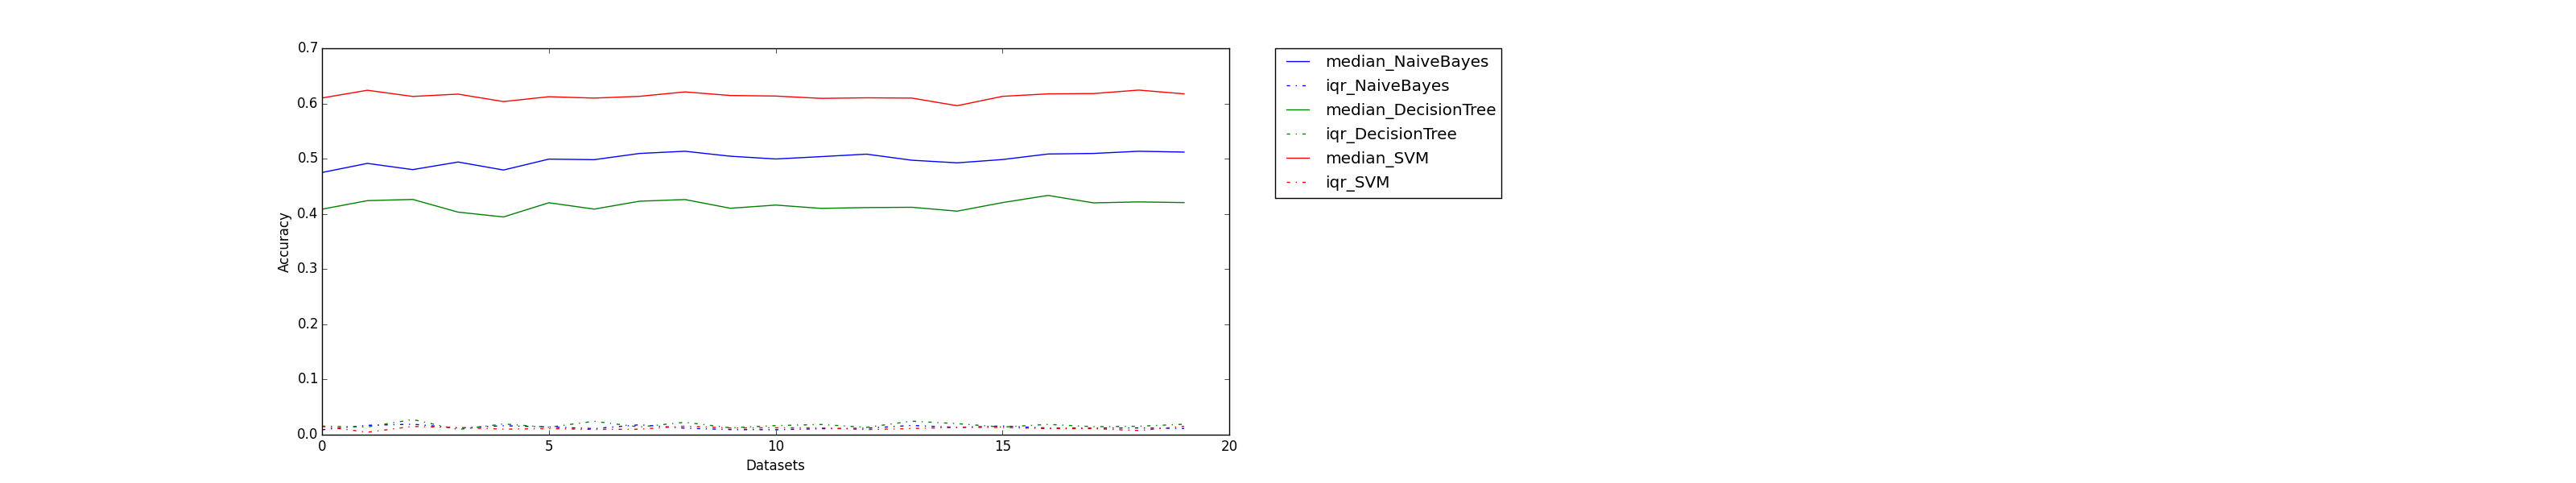
\includegraphics[width=\linewidth]{./fig/algms_smote_acc.png}
        \label{fig:algms_smote_acc}
    }
    \quad
    \subfigure[$Fscore_{M}$]
    {
        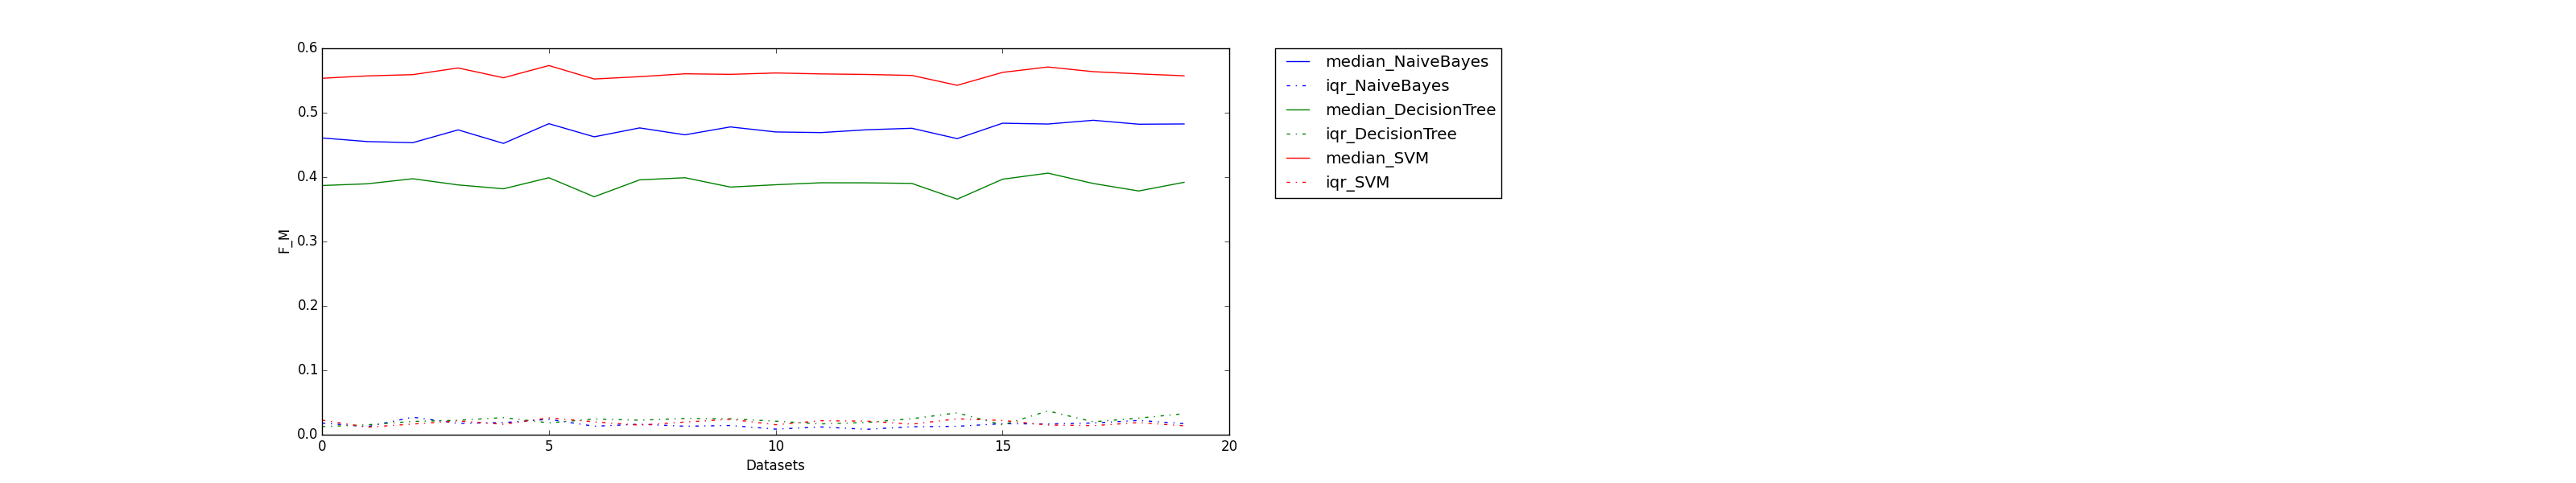
\includegraphics[width=\linewidth]{./fig/algms_smote_M.png}
        \label{fig:algms_smote_M}
    }
    \quad
    \subfigure[$Fscore_{\mu}$]
    {
        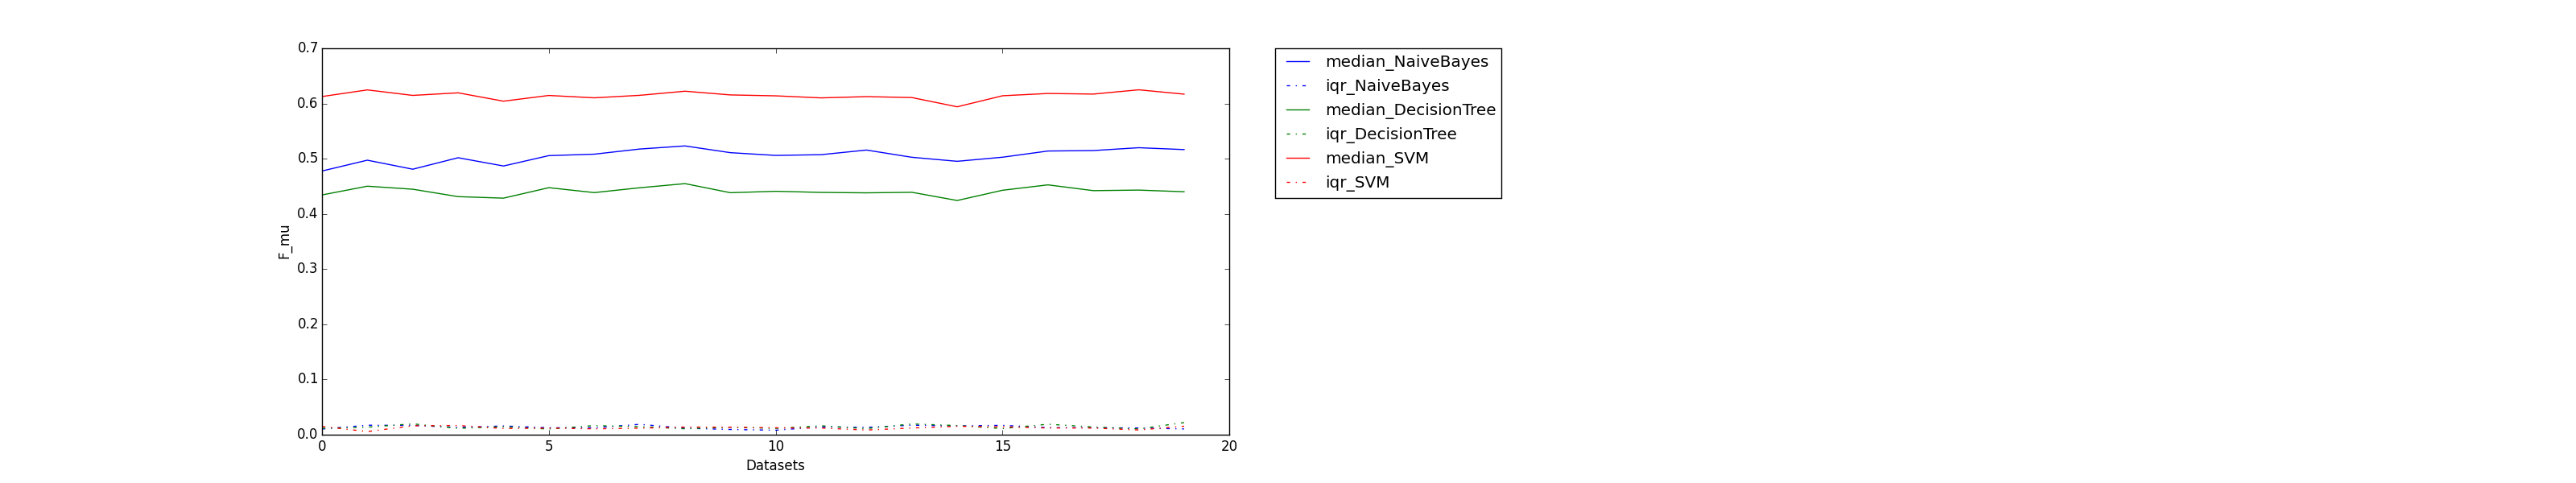
\includegraphics[width=\linewidth]{./fig/algms_smote_mu.png}
        \label{fig:algms_smote_mu}
    }
    \caption{SVM versus Naive Bayes versus CART}
    \label{fig:algms}
\end{figure}

As shown in Figure \ref{fig:algms}, linear SVM outperforms all the others because of the high dimensionality of the data.

\section{Discussion}
\label{sec:Discussion}

The best practice we get has scores of accuracy: 0.613, $Fscore_{M}$: 0.560, $Fscore_{\mu}$: 0.614. It is better than the results of Kuo \cite{kuo2011word} and Moharana \cite{moharanatag} but the approach of Clayton and Byrne \cite{stanley2013predicting} got a higher accuracy. Possible reasons are...

\textbf{RQ4} How can we further improve the performance?

More decisions can always be explored in each step (tokenization, featurization, etc.). However, the most promising improvement can be the implementation of specific preprocessing for Software Engineering text. The most significant feature of Software Engineering text is that it usually contains codes. Analysis of this codes can provide additional information for the text categorization problem.

\subsection{Validity threats}

There are several validity threats to the design of this study. First, limited number of text mining decisions are explored, which cannot represent the whole decision space. Second, a greedy search is implemented to explore the limited decision space, which makes the best practice a satisfactory solution instead of a global optimal solution. Last, data we use is part of the entire StackOverflow data. Scalability can be a problem if we want to implement our method on the entire StackOverflow data set, which contains ten million posts.

\section{Conclusions}
\label{sec:Conclusions}



%ACKNOWLEDGMENTS are optional
\section{Acknowledgments}


%
% The following two commands are all you need in the
% initial runs of your .tex file to
% produce the bibliography for the citations in your paper.
\bibliographystyle{abbrv}
\bibliography{sigproc}  % sigproc.bib is the name of the Bibliography in this case
% You must have a proper ".bib" file
%  and remember to run:
% latex bibtex latex latex
% to resolve all references
%
% ACM needs 'a single self-contained file'!
%
\end{document}
